\PassOptionsToPackage{enable-debug,check-declarations}{expl3}
\RequirePackage{pdfmanagement-testphase}
\DeclareDocumentMetadata {  }
\ExplSyntaxOn
\pdfmanagement_add:nnn{Catalog}{Lang}{(enUS)}
\ExplSyntaxOff

% xmp metadata for pdf
% Originally used \usepackage[a-2a]{pdfx}
% \usepackage{hyperxmp} replaced it
% \RequirePackage{pdfmanagement-testphase} replaced it

\documentclass[11pt,
  english,
  letterpaper,
]{article}
\usepackage{sa4ss}
\usepackage{amsmath,amssymb,array}
\usepackage{booktabs}

% From tagged-template.latex
\usepackage{lmodern}
\usepackage{ifxetex,ifluatex}
\ifnum 0\ifxetex 1\fi\ifluatex 1\fi=0 % if pdftex
  \usepackage[T1]{fontenc}
  \usepackage[utf8]{inputenc}
  \usepackage{textcomp} % provide euro and other symbols
\else % if luatex or xetex
  \usepackage{unicode-math}
  \defaultfontfeatures{Scale=MatchLowercase}
  \defaultfontfeatures[\rmfamily]{Ligatures=TeX,Scale=1}
\fi

% Use upquote if available, for straight quotes in verbatim environments
\IfFileExists{upquote.sty}{\usepackage{upquote}}{}
\IfFileExists{microtype.sty}{% use microtype if available
  \usepackage[]{microtype}
  \UseMicrotypeSet[protrusion]{basicmath} % disable protrusion for tt fonts
}{}
\makeatletter
\@ifundefined{KOMAClassName}{% if non-KOMA class
  \IfFileExists{parskip.sty}{%
    \usepackage{parskip}
  }{% else
    \setlength{\parindent}{0pt}
    \setlength{\parskip}{6pt plus 2pt minus 1pt}}
}{% if KOMA class
  \KOMAoptions{parskip=half}}
\makeatother
\usepackage{xcolor}
\IfFileExists{xurl.sty}{\usepackage{xurl}}{} % add URL line breaks if available
\hypersetup{
  pdftitle={Evaluating available information to inform stock management delineation for quillback rockfish (Sebastes maliger) off the U.S. West coast},
  pdflang={en},
  hidelinks,
  pdfcreator={LaTeX via pandoc}}
\urlstyle{same} % disable monospaced font for URLs
\usepackage{longtable}
% Correct order of tables after \paragraph or \subparagraph
\usepackage{etoolbox}
\makeatletter
\patchcmd\longtable{\par}{\if@noskipsec\mbox{}\fi\par}{}{}
\makeatother
% Allow footnotes in longtable head/foot
\IfFileExists{footnotehyper.sty}{\usepackage{footnotehyper}}{\usepackage{footnote}}
\makesavenoteenv{longtable}
\usepackage{graphicx}
\makeatletter
\def\maxwidth{\ifdim\Gin@nat@width>\linewidth\linewidth\else\Gin@nat@width\fi}
\def\maxheight{\ifdim\Gin@nat@height>\textheight\textheight\else\Gin@nat@height\fi}
\makeatother
% Scale images if necessary, so that they will not overflow the page
% margins by default, and it is still possible to overwrite the defaults
% using explicit options in \includegraphics[width, height, ...]{}
\setkeys{Gin}{width=\maxwidth,height=\maxheight,keepaspectratio}
% Set default figure placement to htbp
\makeatletter
\def\fps@figure{htbp}
\makeatother
\setlength{\emergencystretch}{3em} % prevent overfull lines
\providecommand{\tightlist}{%
  \setlength{\itemsep}{0pt}\setlength{\parskip}{0pt}}
\setcounter{secnumdepth}{5}
\ifxetex
  % Load polyglossia as late as possible: uses bidi with RTL langages (e.g. Hebrew, Arabic)
  \usepackage{polyglossia}
  \setmainlanguage[]{english}
\else
  \usepackage[shorthands=off,main=english]{babel}
\fi

%Define cslreferences environment, required by pandoc 2.8
%https://github.com/rstudio/rmarkdown/issues/1649


\providecommand{\tightlist}{%
  \setlength{\itemsep}{0pt}\setlength{\parskip}{0pt}}


\date{}
\newcommand{\trTitle}{Evaluating available information to inform stock management delineation for quillback rockfish (\emph{Sebastes maliger}) off the U.S. West coast}
\newcommand{\trYear}{2021}
\newcommand{\trMonth}{October}
\newcommand{\trAuthsLong}{true}
\newcommand{\trAuthsBack}{Langseth, B.J., C.R. Wetzel}
\newcommand{\trCitation}{
\begin{hangparas}{1em}{1}
\trAuthsBack{}. \trYear{}. \trTitle{}. \glsentrylong{pfmc}, Portland, Oregon. \pageref{LastPage}{}\,p.
\end{hangparas}}

\AtBeginDocument{\tagstructbegin{tag=Document}}
\AtEndDocument{\tagstructend}
\pretocmd{\maketitle}{\tagstructbegin{tag=H1}\tagmcbegin{tag=H1}}{}{}
\apptocmd{\maketitle}{\tagmcend\tagstructend}{}{}

\begin{document}

%%%%% Frontmatter %%%%%

% Footnote symbols in front matter
\renewcommand*{\thefootnote}{\fnsymbol{footnote}}

\small
\thispagestyle{empty}
\pagenumbering{roman}
\noindent
\begin{center}
\title{Evaluating available information to inform stock management delineation for quillback rockfish (\emph{Sebastes maliger}) off the U.S. West coast}
% \textnormal{\MakeTextUppercase{\trTitle{}}}
\vspace{1.5cm}
{\Large\textbf\newline{Evaluating available information to inform stock management delineation for quillback rockfish (\emph{Sebastes maliger}) off the U.S. West coast}}
\vfill
by\\
Brian J. Langseth\textsuperscript{1}\\
Chantel R. Wetzel\textsuperscript{1}\vfill
\textsuperscript{1}Northwest Fisheries Science Center, U.S. Department of Commerce, National Oceanic and Atmospheric Administration, National Marine Fisheries Service, 2725 Montlake Boulevard East, Seattle, Washington 98112\vfill
\trMonth{} \trYear{}
\end{center}
\clearpage

% Fourth page: Colophon
\thispagestyle{empty}
\vspace*{\fill}
\begin{center}
\copyright{} \glsentrylong{pfmc}, \trYear{}\\
\end{center}
\par
\bigskip
\noindent
Correct citation for this publication:
\bigskip
\par
\trCitation{}
\clearpage

% Add TOC to pdf bookmarks (clickable pdf)
\pdfbookmark[1]{\contentsname}{toc}

% Table of contents page, lists of figures and tables
\tableofcontents\clearpage
\label{TRlastRoman}
\clearpage

% Table of contents
\newpage
\thispagestyle{empty} % to remove page number

% Settings for the main document
\pagenumbering{arabic}  % Regular page numbers
\pagestyle{plain}  % No page number on first page of main document, use 'empty'
\renewcommand*{\thefootnote}{\arabic{footnote}}  % Back to numeric footnotes
\setcounter{footnote}{0}  % And start at 1
\renewcommand{\headrulewidth}{0.5pt}
\renewcommand{\footrulewidth}{0.5pt}
%\pagestyle{fancy}\fancyhead[c]{Draft: Do not cite or circulate}

\newcommand{\lt}{\ensuremath <}
\newcommand{\gt}{\ensuremath >}

\pagebreak
\pagenumbering{roman}
\setcounter{page}{1}

\renewcommand{\thetable}{\roman{table}}
\renewcommand{\thefigure}{\roman{figure}}

\setlength\parskip{0.5em plus 0.1em minus 0.2em}

\pagebreak
\setlength{\parskip}{5mm plus1mm minus1mm}
\pagenumbering{arabic}
\setcounter{page}{1}
\renewcommand{\thefigure}{\arabic{figure}}
\renewcommand{\thetable}{\arabic{table}}
\setcounter{table}{0}
\setcounter{figure}{0}

\setlength\parskip{0.2em plus 0.1em minus 0.2em}

\tagstructbegin{tag=H1}\tagmcbegin{tag=H1}

\hypertarget{introduction}{%
\section{Introduction}\label{introduction}}

\leavevmode\tagmcend\tagstructend

\tagstructbegin{tag=P}\tagmcbegin{tag=P}

At the September 2021 Council meeting, the Council requested that the Groundfish Subcommittee (GFSC) evaluate and make recommendations on the stock delineations for copper, quillback, and vermillion/sunset rockfish. Information for copper rockfish was presented at the GFSC mop-up meeting on September 29-30, 2021 {\tagstructbegin{tag=Reference}\tagmcbegin{tag=Reference}(Wetzel 2021)\leavevmode\tagmcend\tagstructend}. This report updates the information prepared for copper rockfish for application to quillback rockfish. There are relatively few directed studies on quillback rockfish compared to copper rockfish, so focusing on quillback rockfish adds limited information beyond that already provided for copper rockfish. To more clearly indicate the information most applicable to quillback rockfish, we have added text to the beginning of the study descriptions to clarify studies that focus on or include quillback rockfish.

\leavevmode\tagmcend\tagstructend\par

\tagstructbegin{tag=H1}\tagmcbegin{tag=H1}

\hypertarget{status-determination-across-area-based-assessments}{%
\section{Status determination across area-based assessments}\label{status-determination-across-area-based-assessments}}

\leavevmode\tagmcend\tagstructend

\tagstructbegin{tag=H2}\tagmcbegin{tag=H2}

\hypertarget{dispersal}{%
\subsection{Dispersal}\label{dispersal}}

\leavevmode\tagmcend\tagstructend

\tagstructbegin{tag=H3}\tagmcbegin{tag=H3}

\hypertarget{recruitment-and-dispersal}{%
\subsubsection{Recruitment and Dispersal}\label{recruitment-and-dispersal}}

\leavevmode\tagmcend\tagstructend

\tagstructbegin{tag=P}\tagmcbegin{tag=P}

\emph{Evidence for Managing at Assessment Scale}

\leavevmode\tagmcend\tagstructend\par

\tagstructbegin{tag=P}\tagmcbegin{tag=P}

Markel {\tagstructbegin{tag=Reference}\tagmcbegin{tag=Reference}(2011)\leavevmode\tagmcend\tagstructend} - quillback included: Observed significant differences of recruitment in rockfish species among sites and years which were not consistent, indicating spatial differences in recruitment intensity during year of high recruitment within the Barkley Sound, British Columbia. Study was based on black rockfish, and a complex of copper, quillback, and brown rockfish.

\leavevmode\tagmcend\tagstructend\par

\tagstructbegin{tag=P}\tagmcbegin{tag=P}

Sivasundar and Palumbi {\tagstructbegin{tag=Reference}\tagmcbegin{tag=Reference}(2010)\leavevmode\tagmcend\tagstructend} - general rockfish: Have a schematic (their Figure 1) that shows a general ecological gradient from weak upwelling and high larval settlement in waters off Oregon/Washington to strong upwelling and low larval settlement in waters near Point Conception, California.

\leavevmode\tagmcend\tagstructend\par

\tagstructbegin{tag=P}\tagmcbegin{tag=P}

\emph{Evidence for Alternative Management Scale}

\leavevmode\tagmcend\tagstructend\par

\tagstructbegin{tag=P}\tagmcbegin{tag=P}

No studies were found that included quillback rockfish.

\leavevmode\tagmcend\tagstructend\par

\tagstructbegin{tag=P}\tagmcbegin{tag=P}

\emph{Information from assessment reports}

\leavevmode\tagmcend\tagstructend\par

\tagstructbegin{tag=P}\tagmcbegin{tag=P}

Quillback assessment: Annual recruitment deviations were estimated in the base models for California and Oregon, but not Washington. Overlaying recruitment estimates across areas (using the model sensitivity to estimating annual recruitment deviations for Washington) showed some general coherence with the overall patterns of positive or negative recruitment deviations among areas, with variability in individual years (Figure \ref{fig:recruit-comparison}). In the base model for Washington we opted to not estimate annual recruitment deviations due to limited information available in the length compositions for that area). \emph{Caveat}: Length data may not be fully informative for recruitment as variation in growth can result in low or high recruitment years being attributed to multiple years.

\leavevmode\tagmcend\tagstructend\par

\tagstructbegin{tag=Figure,alttext={.}}\tagmcbegin{tag=Figure}

\begin{figure}
\centering
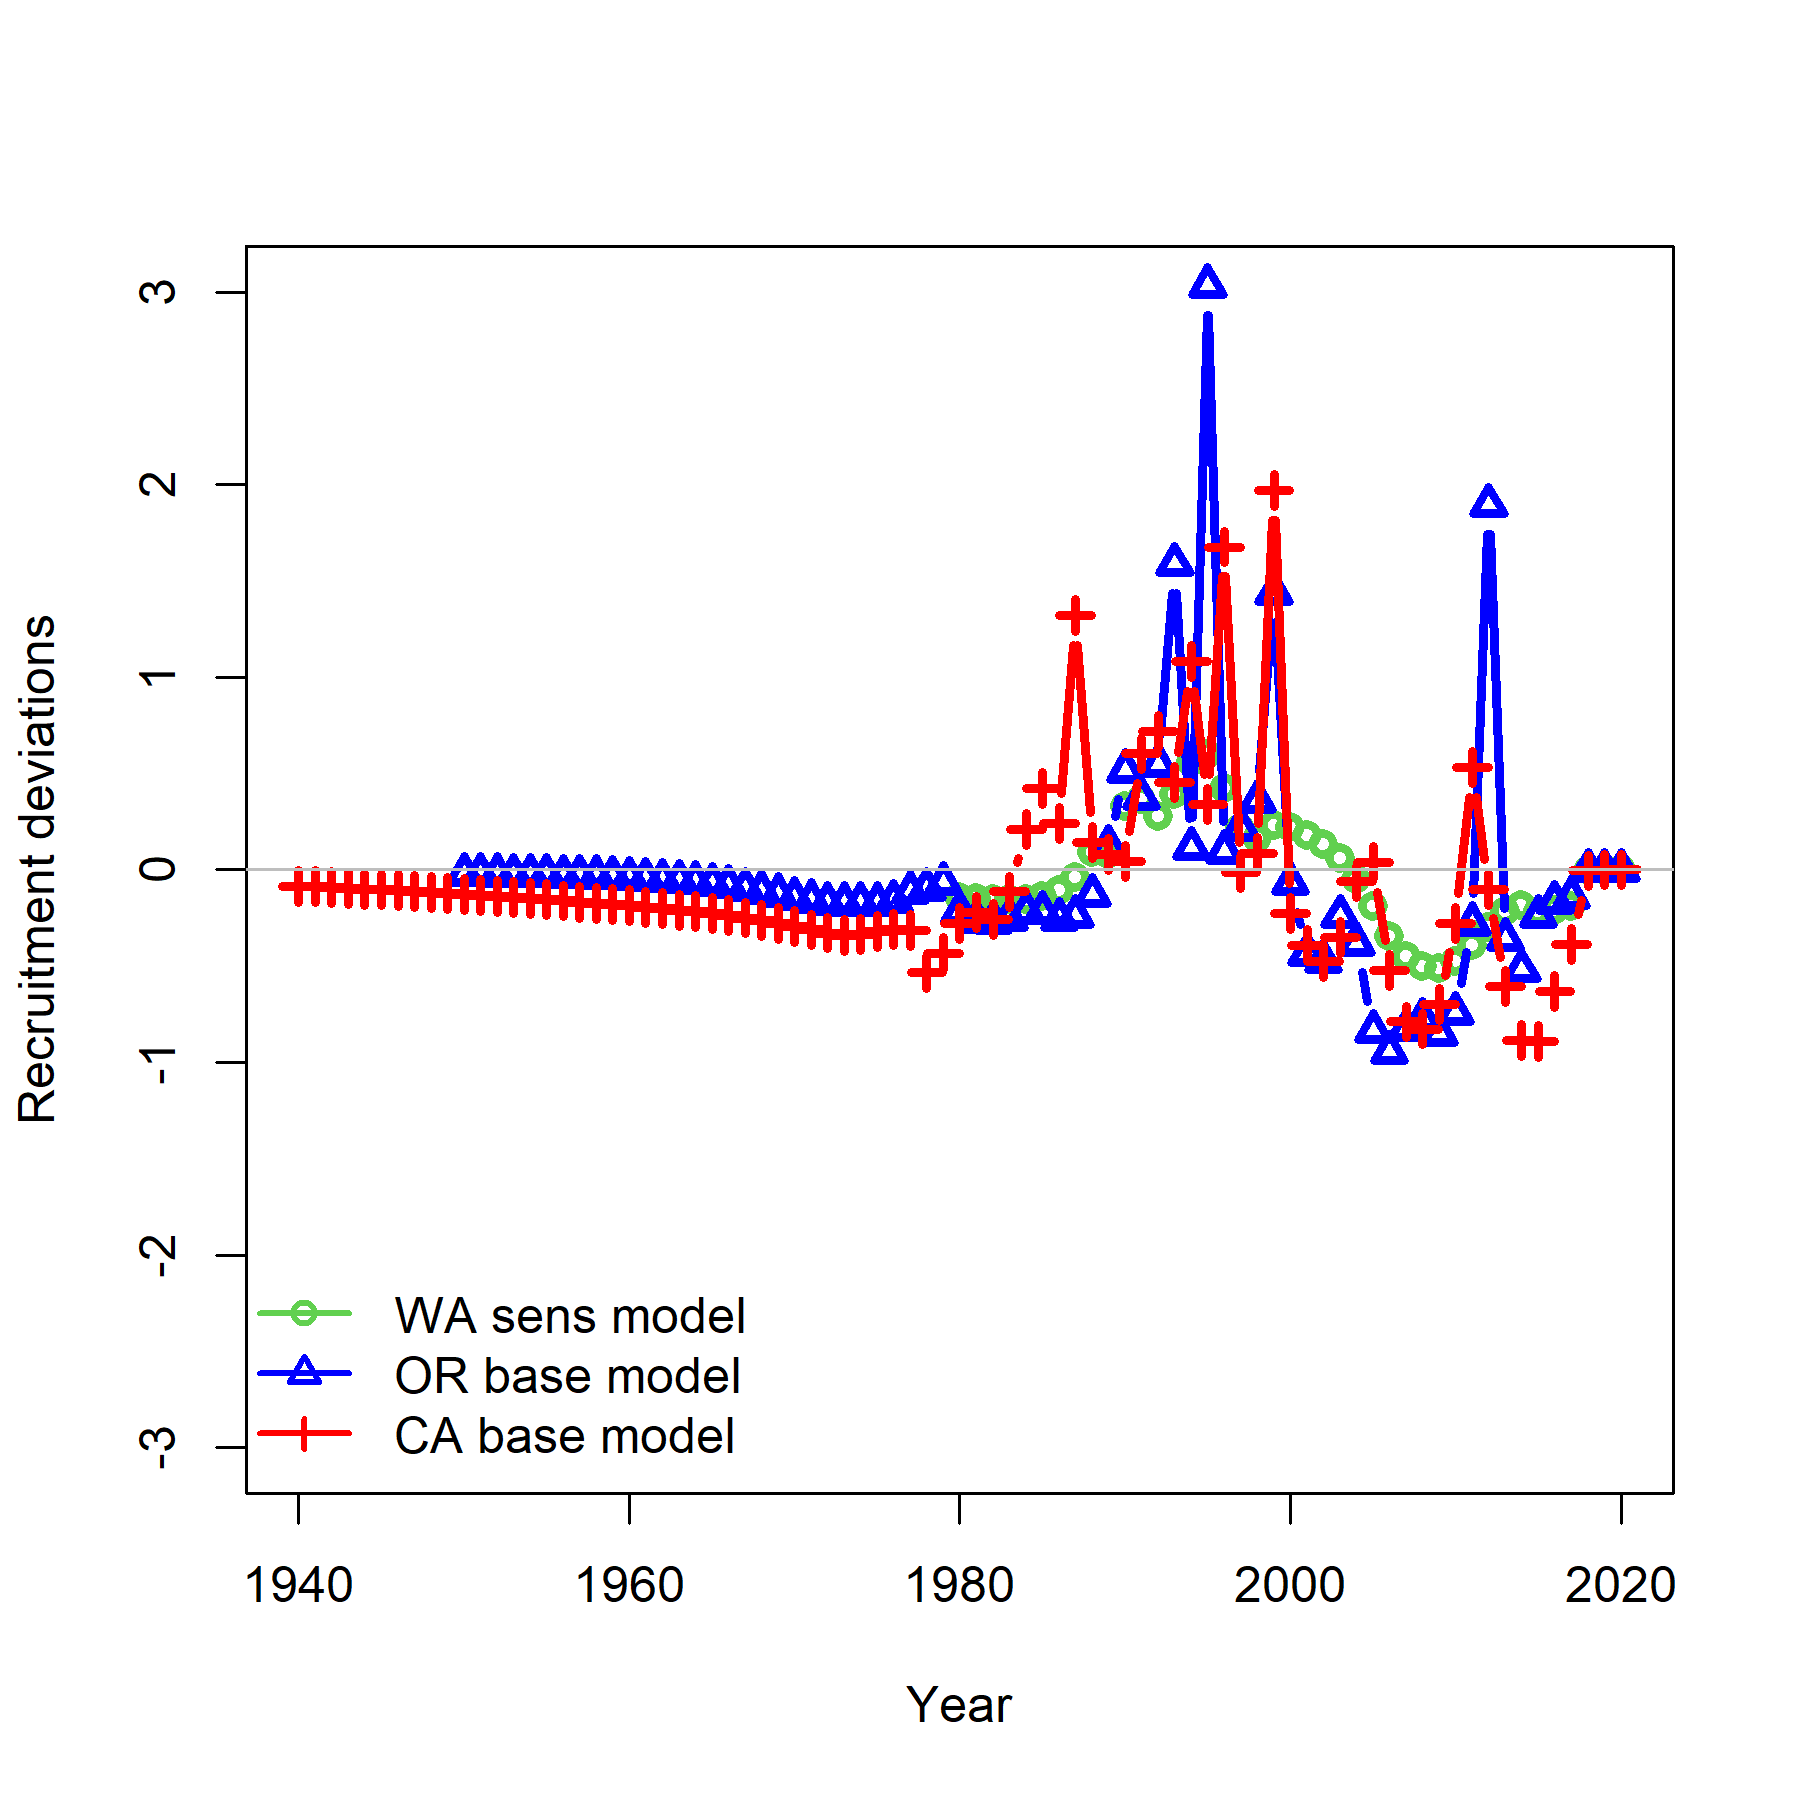
\includegraphics[width=1\textwidth,height=1\textheight]{comprare_recruitments.png}
\caption{Estimates of recruitment in millions of eggs from the base models for Oregon and California, and from the sensitivity where recruitment was estimated for Washington.\label{fig:recruit-comparison}}
\end{figure}

\tagmcend\tagstructend

\tagstructbegin{tag=H3}\tagmcbegin{tag=H3}

\hypertarget{adult-movement}{%
\subsubsection{Adult Movement}\label{adult-movement}}

\leavevmode\tagmcend\tagstructend

\tagstructbegin{tag=P}\tagmcbegin{tag=P}

\emph{Evidence for Managing at Assessment Scale}

\leavevmode\tagmcend\tagstructend\par

\tagstructbegin{tag=P}\tagmcbegin{tag=P}

Matthews {\tagstructbegin{tag=Reference}\tagmcbegin{tag=Reference}(1990a)\leavevmode\tagmcend\tagstructend} - quillback focused: Home ranges of four tagged quillback rockfish and 11 tagged copper rockfish in Puget Sound, Washington were \textless10m{\tagstructbegin{tag=Formula}\tagmcbegin{tag=Formula}\(^2\)\leavevmode\tagmcend\tagstructend} on high relief reefs but greater (4000m{\tagstructbegin{tag=Formula}\tagmcbegin{tag=Formula}\(^2\)\leavevmode\tagmcend\tagstructend}) on low relief reefs. Quillback rockfish exhibited long periods of residency with limited movements. A study with substantially more samples based on copper, quillback, and brown rockfish {\tagstructbegin{tag=Reference}\tagmcbegin{tag=Reference}(Matthews 1990b)\leavevmode\tagmcend\tagstructend} indicated similar patterns with ranges 30m{\tagstructbegin{tag=Formula}\tagmcbegin{tag=Formula}\(^2\)\leavevmode\tagmcend\tagstructend}-1500m{\tagstructbegin{tag=Formula}\tagmcbegin{tag=Formula}\(^2\)\leavevmode\tagmcend\tagstructend} depending on reef type and season.

\leavevmode\tagmcend\tagstructend\par

\tagstructbegin{tag=P}\tagmcbegin{tag=P}

Tolimieri et al.~{\tagstructbegin{tag=Reference}\tagmcbegin{tag=Reference}(2009)\leavevmode\tagmcend\tagstructend} - quillback focused: Observed that home ranges of quillback rockfish in Puget Sound, Washington were relatively small (\textasciitilde1500m{\tagstructbegin{tag=Formula}\tagmcbegin{tag=Formula}\(^2\)\leavevmode\tagmcend\tagstructend} to \textasciitilde2500m{\tagstructbegin{tag=Formula}\tagmcbegin{tag=Formula}\(^2\)\leavevmode\tagmcend\tagstructend}) and similar among copper and quillback rockfish and lingcod. Caveat: movement of fish in the Puget Sound may not be representative of movement in coastal populations.

\leavevmode\tagmcend\tagstructend\par

\tagstructbegin{tag=P}\tagmcbegin{tag=P}

Hannah and Rankin {\tagstructbegin{tag=Reference}\tagmcbegin{tag=Reference}(2011)\leavevmode\tagmcend\tagstructend} - quillback included: Observed high site fidelity for quillback rockfish based on tagging of four individuals tracked for approximately one year within a 5,200 ha study area. Vermilion, china, tiger, and some yelloweye rockfish also showed high site fidelity. In contrast, canary rockfish showed low site fidelty, with home ranges greater than the size of the study area. Black and copper rockfish showed intermediate site fidelity, between that of canary rockfish (low fidelity) and species with high site fidelity.

\leavevmode\tagmcend\tagstructend\par

\tagstructbegin{tag=P}\tagmcbegin{tag=P}

Rankin et al.~{\tagstructbegin{tag=Reference}\tagmcbegin{tag=Reference}(2013)\leavevmode\tagmcend\tagstructend} - quillback included: Observed larger home ranges of quillback and copper rockfish than found in previous studies based on tagging and telemetry of 9 quillback rockfish and 8 copper rockfish at Cape Pertetua Reef, Oregon. Home ranges were approximately 1200m{\tagstructbegin{tag=Formula}\tagmcbegin{tag=Formula}\(^2\)\leavevmode\tagmcend\tagstructend}-8000m{\tagstructbegin{tag=Formula}\tagmcbegin{tag=Formula}\(^2\)\leavevmode\tagmcend\tagstructend} for most individuals, with one quillback rockfish extending out to 24,000m{\tagstructbegin{tag=Formula}\tagmcbegin{tag=Formula}\(^2\)\leavevmode\tagmcend\tagstructend}. Found that hypoxic conditions reduced copper rockfish home ranges approximately 33\% but not quillback rockfish home ranges.

\leavevmode\tagmcend\tagstructend\par

\tagstructbegin{tag=P}\tagmcbegin{tag=P}

Lea et al {\tagstructbegin{tag=Reference}\tagmcbegin{tag=Reference}(1999)\leavevmode\tagmcend\tagstructend} - quillback mentioned: Summarized tagging data from Morro to Monterey Bays, California that reported species of the gopher complex (which includes quillback rockfish although no quillback rockfish data were provided) to have no movement and therefore considered very residential in California. Blue, black, olive, and vermilion rockfish were also considered to have high site fidelity. Copper rockfish was found to have limited movement as were gopher and olive rockfish. Of 32 tagged copper rockfish that were recaptured the distance moved ranged between 0-1.5 nautical miles after 2-1,017 days at liberty. Canary and yellowtail rockfish, and lingcod showed capacity for moving great distances.

\leavevmode\tagmcend\tagstructend\par

\tagstructbegin{tag=P}\tagmcbegin{tag=P}

\emph{Evidence for Alternative Management Scale}

\leavevmode\tagmcend\tagstructend\par

\tagstructbegin{tag=P}\tagmcbegin{tag=P}

No studies were found that included quillback rockfish.

\leavevmode\tagmcend\tagstructend\par

\tagstructbegin{tag=H2}\tagmcbegin{tag=H2}

\hypertarget{geographic-variation}{%
\subsection{Geographic variation}\label{geographic-variation}}

\leavevmode\tagmcend\tagstructend

\tagstructbegin{tag=H3}\tagmcbegin{tag=H3}

\hypertarget{variation-in-genetic-composition}{%
\subsubsection{Variation in Genetic Composition}\label{variation-in-genetic-composition}}

\leavevmode\tagmcend\tagstructend

\tagstructbegin{tag=P}\tagmcbegin{tag=P}

\emph{Evidence for Managing at Assessment Scale}

\leavevmode\tagmcend\tagstructend\par

\tagstructbegin{tag=P}\tagmcbegin{tag=P}

No studies were found that included quillback rockfish.

\leavevmode\tagmcend\tagstructend\par

\tagstructbegin{tag=P}\tagmcbegin{tag=P}

\emph{Evidence for Alternative Management Scale}

\leavevmode\tagmcend\tagstructend\par

\tagstructbegin{tag=P}\tagmcbegin{tag=P}

Seeb {\tagstructbegin{tag=Reference}\tagmcbegin{tag=Reference}(1998)\leavevmode\tagmcend\tagstructend} - quillback focused: Significant genetic differences were found between Puget Sound and coastal stocks of quillback rockfish based on allozyme frequency and mtDNA, however there was not significant differentiation in allozyme frequency in populations of quillback rockfish between coastal Washington and Alaska. \emph{Caveat}: This study would fall under ``evidence for managing at assessment scales'' for copper or brown rockfish as significant differentiation was found for copper rockfish across the range of the study (California to Alaska) based on both allozyme frequency and mtDNA. Significant differences in allozyme frequency (but not mtDNA) were found for brown rockfish between Washington and California.

\leavevmode\tagmcend\tagstructend\par

\tagstructbegin{tag=P}\tagmcbegin{tag=P}

\emph{Caveat}

\leavevmode\tagmcend\tagstructend\par

\tagstructbegin{tag=P}\tagmcbegin{tag=P}

Stout et al.~{\tagstructbegin{tag=Reference}\tagmcbegin{tag=Reference}(2001)\leavevmode\tagmcend\tagstructend} - quillback focused: Concluded there were three distinct population sub-units of quillback rockfish within Puget Sound, Washington. Relied heavily on information from the genetic studies of Seeb {\tagstructbegin{tag=Reference}\tagmcbegin{tag=Reference}(1998)\leavevmode\tagmcend\tagstructend}.

\leavevmode\tagmcend\tagstructend\par

\tagstructbegin{tag=P}\tagmcbegin{tag=P}

Schwenke et al.~{\tagstructbegin{tag=Reference}\tagmcbegin{tag=Reference}(2018)\leavevmode\tagmcend\tagstructend} - quillback included: Found long-term low-level introgression among quillback, copper, and brown rockfish within the Salish sea at higher rates than in coastal populations. Suggests greater isolation of Salish Sea populations, possibly due to the specific environmental conditions in the sub basins of the Salish Sea. Also could explain some of the differences with Puget Sound quillback rockfish compared to coastal populations.

\leavevmode\tagmcend\tagstructend\par

\tagstructbegin{tag=P}\tagmcbegin{tag=P}

Waples and Gaggiotti {\tagstructbegin{tag=Reference}\tagmcbegin{tag=Reference}(2006)\leavevmode\tagmcend\tagstructend} - general: Significant differences in neutral genetic characters indicate that the populations have been reproductively isolated for many generations, which is far longer than the ecological time scales that are relevant to stock assessment or fishery management. Argue for use of mtDNA data to determine demographic independence on the scales relevant to stock assessment.

\leavevmode\tagmcend\tagstructend\par

\tagstructbegin{tag=H3}\tagmcbegin{tag=H3}

\hypertarget{variation-in-phenotypic-traits}{%
\subsubsection{Variation in Phenotypic Traits}\label{variation-in-phenotypic-traits}}

\leavevmode\tagmcend\tagstructend

\tagstructbegin{tag=P}\tagmcbegin{tag=P}

\emph{Evidence for Managing at Assessment Scale}

\leavevmode\tagmcend\tagstructend\par

\tagstructbegin{tag=P}\tagmcbegin{tag=P}

No studies were found that included quillback rockfish.

\leavevmode\tagmcend\tagstructend\par

\tagstructbegin{tag=P}\tagmcbegin{tag=P}

\emph{Evidence for Alternative Management Scale}

\leavevmode\tagmcend\tagstructend\par

\tagstructbegin{tag=P}\tagmcbegin{tag=P}

Quillback assessment: The assessments for quillback rockfish utilized the same growth, maturity, fecundity, and length-weight relationships across areas. Limited differences in growth based on the original age-length estimates between fish off the Oregon and Washington coast as shown at the data workshop in October, 2020. Limited number of new California samples during reviews considered insufficient to estimate a California curve for comparison. \emph{Caveat}: Spatial gradients of growth across the coast are commonly observed in rockfish or other fish species along the U.S. west coast {\tagstructbegin{tag=Reference}\tagmcbegin{tag=Reference}(Keller et al. 2012, 2018; Gertseva et al. 2017)\leavevmode\tagmcend\tagstructend}.

\leavevmode\tagmcend\tagstructend\par

\tagstructbegin{tag=H2}\tagmcbegin{tag=H2}

\hypertarget{other-considerations}{%
\subsection{Other Considerations}\label{other-considerations}}

\leavevmode\tagmcend\tagstructend

\tagstructbegin{tag=H3}\tagmcbegin{tag=H3}

\hypertarget{abundance-trends}{%
\subsubsection{Abundance Trends}\label{abundance-trends}}

\leavevmode\tagmcend\tagstructend

\tagstructbegin{tag=P}\tagmcbegin{tag=P}

\emph{Evidence for Managing at Assessment Scale}

\leavevmode\tagmcend\tagstructend\par

\tagstructbegin{tag=P}\tagmcbegin{tag=P}

Quillback assessment: The trajectories across all model areas showed varying patterns (Figure \ref{fig:relb-comparison}). The separate models for the modeled areas estimated different stock trajectories with the stock in California declining earlier, and to a greater degree, than in Oregon or Washington. Both Oregon and California display an increase in stock size starting in the early 2000s that differs in the magnitude of increase, while Washington's change in stock size is much more gradual overall, and seemingly opposite to that of Oregon and California in recent years. The model for Washington did not estimate annual recruitment deviations which likely contributes to stock trajectory differences in recent years (where large recruitment pulses in the 1990s led to increases in recent stock size).

\leavevmode\tagmcend\tagstructend\par

\tagstructbegin{tag=Figure,alttext={.}}\tagmcbegin{tag=Figure}

\begin{figure}
\centering
\includegraphics[width=1\textwidth,height=1\textheight]{L:/Assessments/CurrentAssessments/DataModerate_2021/Quillback_Rockfish/presentations/base_comparisonscompare4_Bratio_uncertainty.png}
\caption{Estimated relative spawning output (in millions of eggs) by assessed area.\label{fig:relb-comparison}}
\end{figure}

\tagmcend\tagstructend

\clearpage

\tagstructbegin{tag=P}\tagmcbegin{tag=P}

\emph{Evidence for Alternative Management Scale}

\leavevmode\tagmcend\tagstructend\par

\tagstructbegin{tag=P}\tagmcbegin{tag=P}

The areas of true population variation in relative stock size may not align with the assessment boundaries as currently defined. State based management is likely not the only factor impacting relative stock sizes across the coast where movement, habitat availability, and recruitment patterns likely also influence potential differences in relative stock size.

\leavevmode\tagmcend\tagstructend\par

\tagstructbegin{tag=H3}\tagmcbegin{tag=H3}

\hypertarget{size-and-age-composition}{%
\subsubsection{Size and Age Composition}\label{size-and-age-composition}}

\leavevmode\tagmcend\tagstructend

\tagstructbegin{tag=P}\tagmcbegin{tag=P}

\emph{Evidence for Managing at Assessment Scale}

\leavevmode\tagmcend\tagstructend\par

\tagstructbegin{tag=P}\tagmcbegin{tag=P}

Quillback assessment: Different selectivity curves were estimated between the recreational and commercial fisheries across modeled areas (Figure \ref{fig:selectivity-comparison}). Differences were greater between Oregon and California recreational selectivity than Oregon and Washington. For commercial selectivity, the size at which quillback rockfish began to be selected was similar for Oregon and Washington, but the slope of the selectivity curve was similar for California and Washington.

\leavevmode\tagmcend\tagstructend\par

\tagstructbegin{tag=Figure,alttext={.}}\tagmcbegin{tag=Figure}

\begin{figure}
\centering
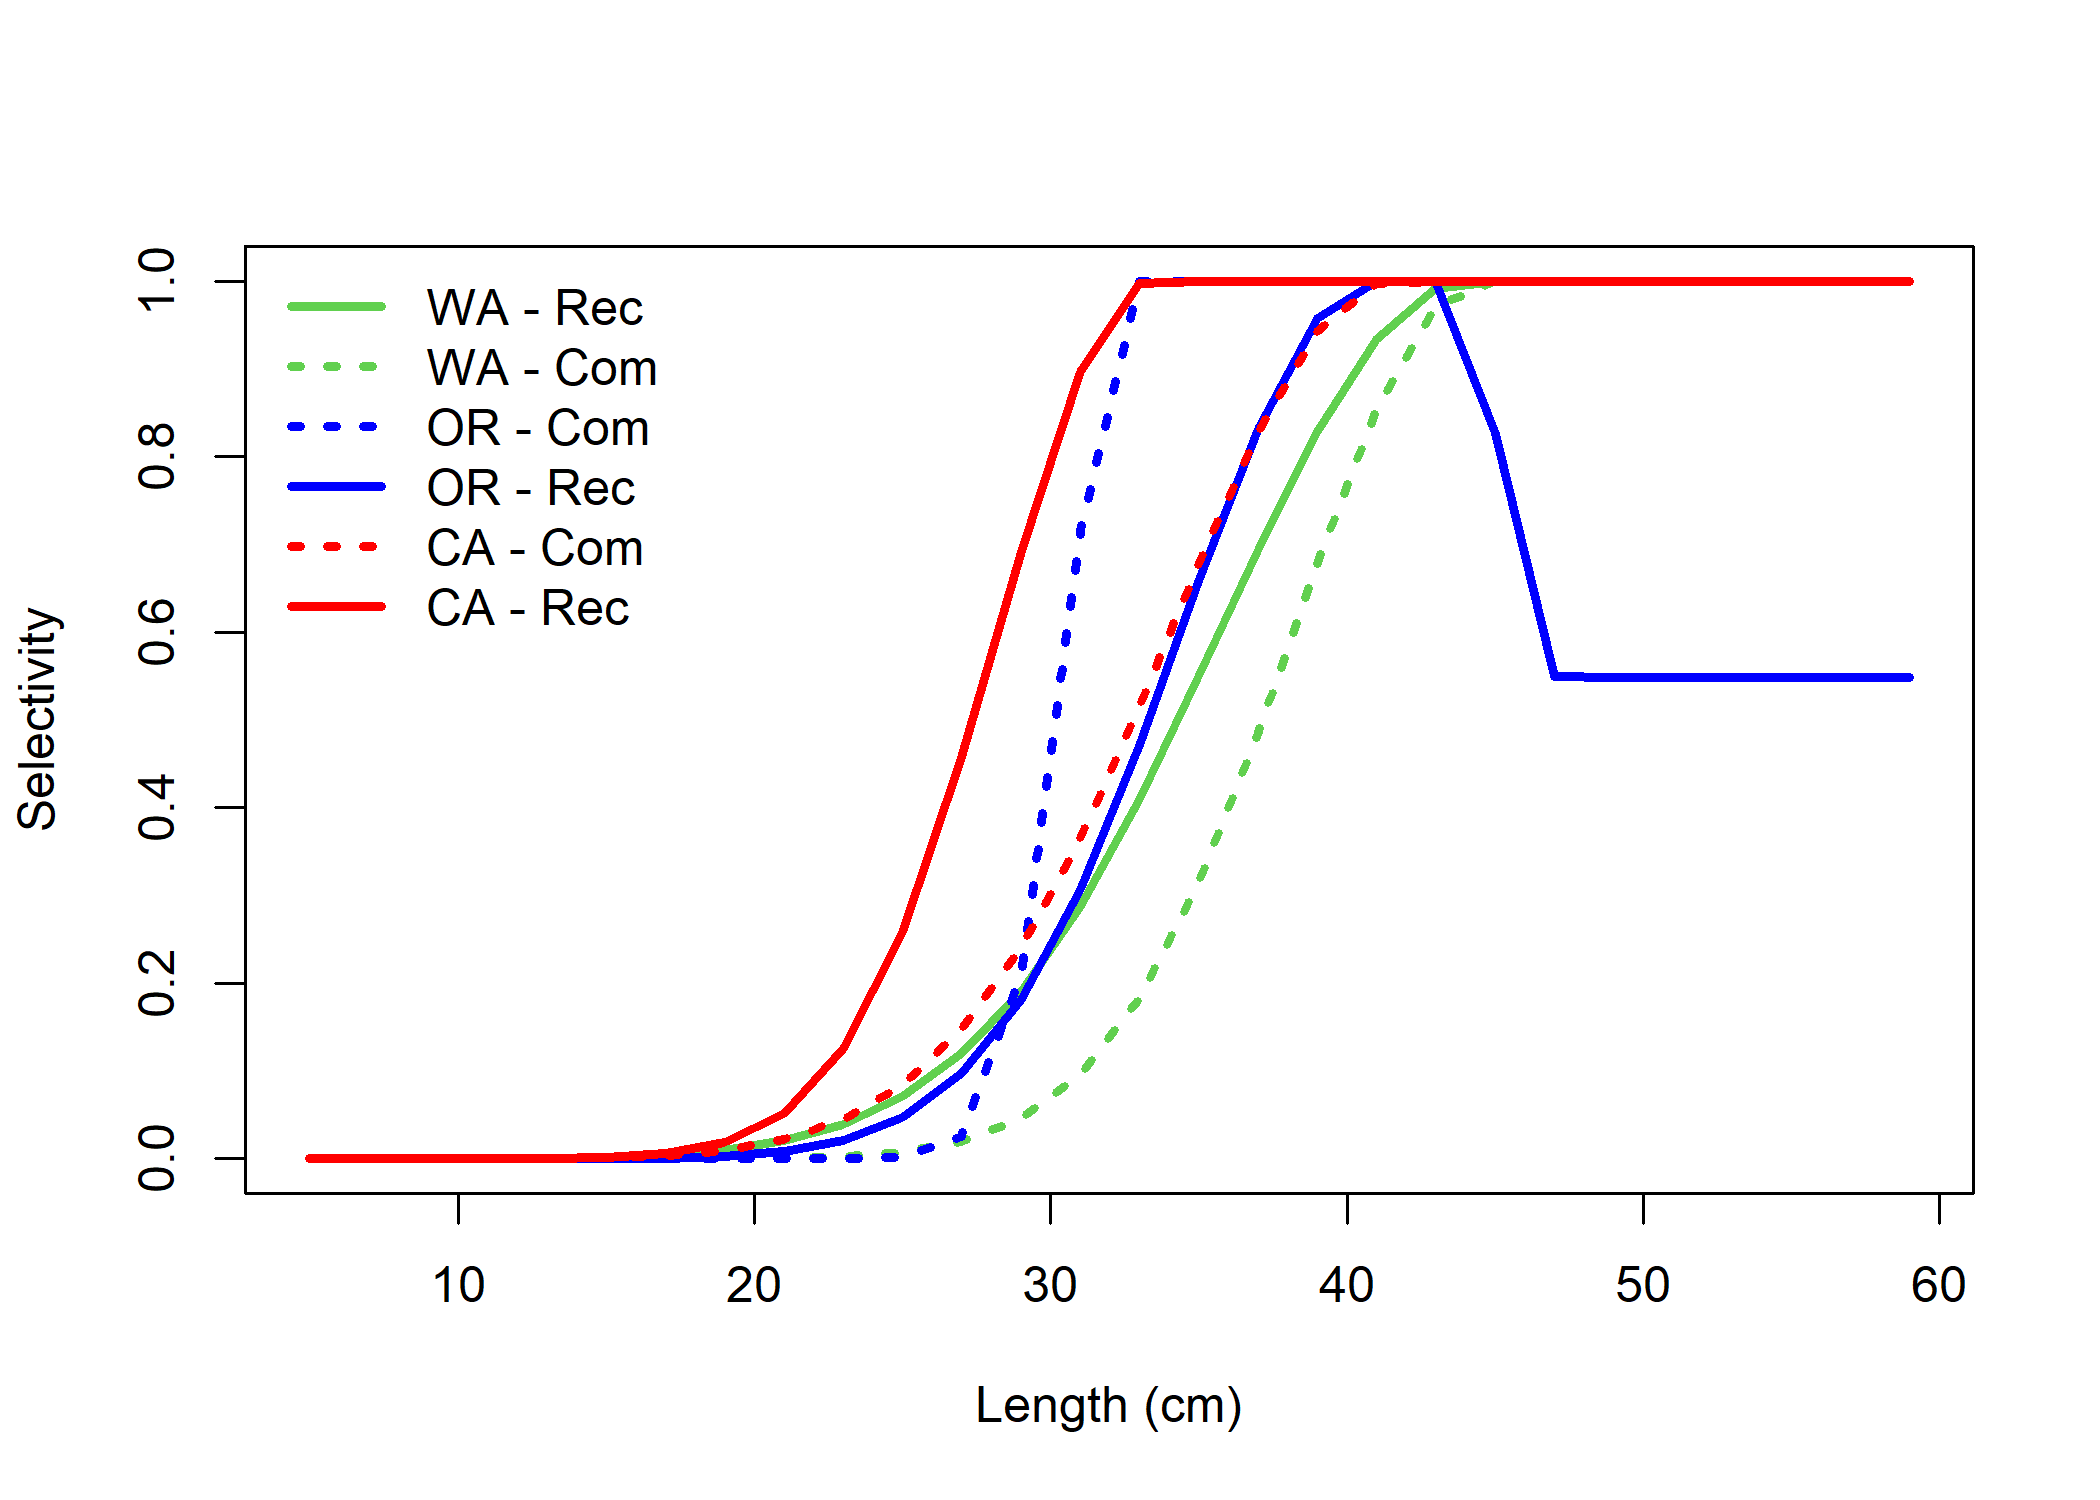
\includegraphics[width=1\textwidth,height=1\textheight]{comprare_selectivity.png}
\caption{Estimated selectivity patterns for commercial (dashed line) and recreational (solid line) fleets by assessed area.\label{fig:selectivity-comparison}}
\end{figure}

\tagmcend\tagstructend

\clearpage

\tagstructbegin{tag=P}\tagmcbegin{tag=P}

Bosely et al.~{\tagstructbegin{tag=Reference}\tagmcbegin{tag=Reference}(2019)\leavevmode\tagmcend\tagstructend} - general: Specifying the correct form of spatial population structure may not be as critical as understanding movement patterns and spatial heterogeneity in fishery selectivity and life-history variation when developing reference points for management.

\leavevmode\tagmcend\tagstructend\par

\tagstructbegin{tag=P}\tagmcbegin{tag=P}

Berger et al.~{\tagstructbegin{tag=Reference}\tagmcbegin{tag=Reference}(2021)\leavevmode\tagmcend\tagstructend} - general: Aligning management assessment areas with underlying population structure and processes is important, especially when fishing mortality is disproportionate to vulnerable biomass among management areas, demographic parameters (growth and maturity) are not homogeneous within management areas, and connectivity (via recruitment or movement) unknowingly exists among management areas. Bias and risk were greater for assessments that incorrectly span multiple population segments compared to assessments that cover a subset of a population segment, and these results were exacerbated when there was connectivity between population segments. \emph{Caveat}: The variation in growth and connectivity between areas via recruitment for quillback rockfish off the West Coast is currently unknown or uncertain.

\leavevmode\tagmcend\tagstructend\par

\tagstructbegin{tag=P}\tagmcbegin{tag=P}

\emph{Evidence for Alternative Management Scale}

\leavevmode\tagmcend\tagstructend\par

\tagstructbegin{tag=P}\tagmcbegin{tag=P}

No studies were found that included quillback rockfish.

\leavevmode\tagmcend\tagstructend\par

\clearpage

\clearpage

\tagstructbegin{tag=H1}\tagmcbegin{tag=H1}

\hypertarget{references}{%
\section{References}\label{references}}

\leavevmode\tagmcend\tagstructend

\tagstructbegin{tag=BibEntry}\tagmcbegin{tag=BibEntry}

\hypertarget{refs}{}
\leavevmode\hypertarget{ref-berger_incoherent_2021}{}%
Berger, A.M., Deroba, J.J., Bosley, K.M., Goethel, D.R., Langseth, B.J., Schueller, A.M., and Hanselman, D.H. 2021. Incoherent dimensionality in fisheries management: Consequences of misaligned stock assessment and population boundaries. ICES Journal of Marine Science 78(1): 155--171.

\leavevmode\hypertarget{ref-bosley_overcoming_2019}{}%
Bosley, K.M., Goethel, D.R., Berger, A.M., Deroba, J.J., Fenske, K.H., Hanselman, D.H., Langseth, B.J., and Schueller, A.M. 2019. Overcoming challenges of harvest quota allocation in spatially structured populations. Fisheries Research 220: 105344.

\leavevmode\hypertarget{ref-gertseva_spatial_2017}{}%
Gertseva, V., Matson, S.E., and Cope, J. 2017. Spatial growth variability in marine fish: Example from Northeast Pacific groundfish. ICES Journal of Marine Science 74(6): 1602--1613.

\leavevmode\hypertarget{ref-HannahandRankin_rockfish_site_fidelity_2011}{}%
Hannah, R.W., and Rankin, P.S. 2011. Site fidelity and movement of eight species of pacific rockfish at a high-relief rocky reef on the oregon coast. North American Journal of Fisheries Management 31: 483--494.

\leavevmode\hypertarget{ref-keller_variation_2012}{}%
Keller, A.A., Molton, K.J., Hicks, A.C., Haltuch, M., and Wetzel, C. 2012. Variation in age and growth of greenstriped rockfish (Sebastes elongatus) along the U.S. West coast (Washington to California). Fisheries Research 119-120: 80--88.

\leavevmode\hypertarget{ref-keller_canary_2018}{}%
Keller, A., Frey, P., Wallace, J., Head, M., Wetzel, C., Cope, J., and Harms, J. 2018. Canary rockfishes Sebastes pinniger return from the brink: Catch, distribution and life history along the US west coast (Washington to California). Marine Ecology Progress Series 599: 181--200.

\leavevmode\hypertarget{ref-lea_biological_1999}{}%
Lea, R.N., McAllister, R.D., and VenTresca, D.A. 1999. Biological sspects of nearshore rockfishes of the genus sebastes from Central California with notes on ecologically related sport fishes. State of California The Resources Agency Department of Fish; Game.

\leavevmode\hypertarget{ref-markel_rockfish_2011}{}%
Markel, R.W. 2011. Rockfish recruitment and trophic dynamics on the west coast of vancouver island: Fishing, ocean, climate, and sea otters. Dissertation, University of British Columbia: 146.

\leavevmode\hypertarget{ref-matthews_telemetry_1990}{}%
Matthews, K.R. 1990a. A telemetric study of the home ranges and homing routes of copper and quillback rockfishes on shallow rocky reefs. Canadian Journal of Zoology 68(11): 2243--2250.

\leavevmode\hypertarget{ref-matthews_seasonal_home_range_1990}{}%
Matthews, K.R. 1990b. An experimental study of the habitat preferences and movement patterns of copper, quillback, and brown rockfishes (sebastes spp.). Environmental Biology of Fishes 29: 161--178.

\leavevmode\hypertarget{ref-Rankinetal_hypoxia_and_fidelity_2013}{}%
Rankin, P.S., Hannah, R.W., and Blume, T.O. 2013. Effect of hypoxia on rockfish movements: Implications for understanding the roles of temperature, toxins and site fidelity. Marine Ecology Progress Series 492: 223--234.

\leavevmode\hypertarget{ref-schwenke_introgression_2018}{}%
Schwenke, P.L., Park, L.K., and Hauser, L. 2018. Introgression among three rockfish species (\emph{sebastes} spp.) in the Salish Sea, northeast Pacific Ocean. PLOS ONE 13(3): e0194068.

\leavevmode\hypertarget{ref-seeb_gene_1998}{}%
Seeb, L.W. 1998. Gene flow and introgression within and among three species of rockfishes, Sebastes auriculatus, \emph{S. Caurinus} and \emph{S. Maliger}. Journal of Heredity 89(5): 393--403.

\leavevmode\hypertarget{ref-sivasundar_life_2010}{}%
Sivasundar, A., and Palumbi, S.R. 2010. Life history, ecology and the biogeography of strong genetic breaks among 15 species of Pacific rockfish, Sebastes. Marine Biology 157(7): 1433--1452.

\leavevmode\hypertarget{ref-Stoutetal_DPS_2001}{}%
Stout, H.A., McCain, B.B., Vetter, R.D., Builder, T.L., Lenarz, W.H., Johnson, L.L., and Methot, R.D. 2001. Status review of copper rockfish (\emph{sebastes caurinus}), quillback rockfish (\emph{s. Maliger}), and brown rockfish (\emph{s. Auriculatus}) in puget sound, washington. NOAA Tech. Memo.

\leavevmode\hypertarget{ref-tolimieri_home_2009}{}%
Tolimieri, N., Andrews, K., Williams, G., Katz, S., and Levin, P. 2009. Home range size and patterns of space use by lingcod, copper rockfish and quillback rockfish in relation to diel and tidal cycles. Marine Ecology Progress Series 380: 229--243.

\leavevmode\hypertarget{ref-waples_what_2006}{}%
Waples, R.S., and Gaggiotti, O. 2006. What is a population? An empirical evaluation of some genetic methods for identifying the number of gene pools and their degree of connectivity. Molecular Ecology 15(6): 1419--1439.

\leavevmode\hypertarget{ref-Wetzel_copper_area_2021}{}%
Wetzel, C.R. 2021. Evaluating available information to determine stock management delineation for copper rockfish (sebastes caurinus) off the u.s. West coast. Pacific Fishery Management Council, 7700 Ambassador Place NE, Suite 200, Portland, OR 97220.

\leavevmode\tagmcend\tagstructend
\end{document}
